\documentclass[12pt, a4paper]{report}
\usepackage[utf8x]{inputenc}
\usepackage[T2A]{fontenc}
\usepackage[english,russian]{babel}

\usepackage{graphicx}
\usepackage{listings}
\usepackage{color}

\usepackage{amsmath}
\usepackage{pgfplots}
\usepackage{url}
\usepackage{flowchart}
\usepackage{float}
\usepackage{tikz}
\usepackage{multirow}
\usepackage{graphicx}
\usepackage[
bookmarks=true, colorlinks=true, unicode=true,
urlcolor=black,linkcolor=black, anchorcolor=black,
citecolor=black, menucolor=black, filecolor=black,
]{hyperref}

\DeclareGraphicsExtensions{.pdf,.png,.jpg,.svg}
\usetikzlibrary{shapes, arrows}

\usepackage{pgfplotstable}

\renewcommand\contentsname{Содержание}

\usepackage{geometry}
\geometry{top=15mm}
\geometry{right=15mm}
\geometry{left=15mm}
\geometry{bottom=20mm}
\geometry{ignorefoot}


\lstset{ %
	language=Matlab,                 % выбор языка для подсветки (здесь это С)
	basicstyle=\small\sffamily, % размер и начертание шрифта для подсветки кода
	numbers=left,               % где поставить нумерацию строк (слева\справа)
	numberstyle=\tiny,           % размер шрифта для номеров строк
	stepnumber=1,                   % размер шага между двумя номерами строк
	numbersep=-5pt,                % как далеко отстоят номера строк от         подсвечиваемого кода
	backgroundcolor=\color{white}, % цвет фона подсветки - используем         \usepackage{color}
	showspaces=false,            % показывать или нет пробелы специальными     отступами
	showstringspaces=false,      % показывать или нет пробелы в строках
	showtabs=false,             % показывать или нет табуляцию в строках
	frame=single,              % рисовать рамку вокруг кода
	tabsize=2,                 % размер табуляции по умолчанию равен 2 пробелам
	captionpos=t,              % позиция заголовка вверху [t] или внизу [b] 
	breaklines=true,           % автоматически переносить строки (да\нет)
	breakatwhitespace=false, % переносить строки только если есть пробел
	escapeinside={\%*}{*)},   % если нужно добавить комментарии в коде
	keywordstyle=\color{blue}\ttfamily,
	stringstyle=\color{red}\ttfamily,
	commentstyle=\color{green}\ttfamily,
	morecomment=[l][\color{magenta}]{\#},
	columns=fullflexible }

\usepackage{titlesec, blindtext, color}
\setcounter{secnumdepth}{-1}
\titleformat{\chapter}[hang]{\LARGE\bfseries}{}{0pt}{\LARGE\bfseries}
\titleformat{\section}{\bfseries\Large}{}{-1cm}{\centering}
\titleformat{\subsection}{\bfseries\normalsize}{}{-1cm}{\centering}



\begin{document}
	
	\begin{titlepage}
		
		\begin{table}[H]
			\centering
			\footnotesize
			\begin{tabular}{cc}
				\multirow{8}{*}{
\includegraphics[scale=0.35]{img/bmstu.jpg}}
				& \\
				& \\
				& \textbf{Министерство науки и высшего образования Российской Федерации} \\
				& \textbf{Федеральное государственное бюджетное образовательное учреждение} \\
				& \textbf{высшего образования} \\
				& \textbf{<<Московский государственный технический} \\
				& \textbf{университет имени Н.Э. Баумана>>} \\
				& \textbf{(МГТУ им. Н.Э. Баумана)} \\
				& \textbf{} \\
			\end{tabular}
		\end{table}
		
		\vspace{-2.5cm}
		
		\begin{flushleft}
			\rule[-1cm]{\textwidth}{3pt}
			\rule{\textwidth}{1pt}
		\end{flushleft}
		
		\begin{flushleft}
			\small
			ФАКУЛЬТЕТ
			\underline{<<Информатика и системы управления>>\ \ \ \ \ \ \ 
				\ \ \ \ \ \ \ \ \ \ \ \ \ \ \ \ \ \ \ \ \ \ \ \ \ \ \ \ \ \ \ 
				\ \ \ \ \ \ \ \ \ \ \ \ \ \ \ } \\
			КАФЕДРА
			\underline{<<Программное обеспечение ЭВМ и
				информационные технологии>>
				\ \ \ \ \ \ \ \ \ \ \ \ \ \ \ \ \ \ \ \ }
		\end{flushleft}
		
		\vspace{2cm}
		
		\begin{center}
			\textbf{Лабораторная работа № 1} \\
			\vspace{0.5cm}
			\textbf{Вариант 22}
		\end{center}
		
		\vspace{4cm}
		
		\begin{flushleft}
			\begin{tabular}{ll}
				\textbf{Дисциплина} & Математическая статистика. \\
				\textbf{Тема} & \\
				\textbf{Студент} & Тимонин А. С. \\
				\textbf{Группа} & ИУ7-62Б \\
				\textbf{Оценка (баллы)} & \\
				\textbf{Преподаватель} & Власов П.А. \\
			\end{tabular}
		\end{flushleft}
		
		\vspace{6cm}
		
		\begin{center}
			Москва, 2020 г.
		\end{center}
		
		
	\end{titlepage}
	
	
	\section{Теоретическая часть}
	\subsection{Формулы для вычисления}
	
	\hspace{0.7cm}\textbf{Для генеральной совокупности $\vec{x} = {(x_1, \dots, x_n)}$}
	
	\vspace{0.5cm}\textbf{Формула для вычисления максимального значения $M_{\max}$:}
	
	\begin{equation*} \label{Mmax}
	M_{\max} = \max{(x_1, \dots, x_n)}
	\end{equation*}
	
	\textbf{Формула для вычисления минимального значения $M_{\min}$:}
	
	\begin{equation*} \label{Mmin}
	M_{\min} = \min{(x_1, \dots, x_n)}
	\end{equation*}
	
	\textbf{Размах выборки R  считается по формуле:}
	
	\begin{equation*} \label{R}
	R = M_{\max} - M_{\min}
	\end{equation*}
	
	\textbf{Вычисление оценки математического ожидания MX:}
	
	\begin{equation*}
	\hat{\mu} = \vec{x} = \frac{1}{n}\sum_{i=1}^{n} x_i
	\end{equation*}
	
	\textbf{Вычисление оценки дисперсии DX:}
	
	\begin{equation*}
	S^2 = \frac{1}{n-1} \sum_{i=1}^n (x_i - \overline{x})^2
	\end{equation*}
	
	\vspace{0.5cm}
	\subsection{Определение эмперической плотности и гистограммы}
	
	\hspace{0.5cm} \textbf{Интервальный статистический ряд}
	
	Пусть $\vec{x}$ - выборка из генеральной совокупности X. Если объем n этой выборки велик ($n\geq50$), то значения $x_i$ группируют не только в статистический ряд, но и в так называемый \underline{интервальный статистический ряд}. Для этого отрезок $J = [x_{(1)}, x_{(n))}]$ делят на p равновеликих частей:
	
	\begin{equation*}
	J_i = [a_i,a_{i+1}), i = \overline{0;p-i}
	\end{equation*}
	
	\begin{equation*}
	J_p = [a_{p-1},a_{p}]
	\end{equation*}
	
	\vspace{0.5cm}где $a_i = x_{(1)} + i\Delta,\; t = \overline{0;p}, \Delta = \frac{|J|}{p} = \frac{x_{(n)} - x_{(1)}}{p}$
	
	\vspace{0.5cm}\textbf{\underline{Опр} Интервальным статистическим рядом} называют таблицу
	
	\begin{table}[H]
		\centering
		\begin{tabular}{|c|c|c|c|c|}
			\hline
			$J_1$ & $\dots$ & $J_i$ & $\dots$ & $J_p$ \\
			\hline
			$n_1$ & $\dots$ & $n_i$ & $\dots$ & $n_p$ \\
			\hline
		\end{tabular}
	\end{table}
	
	Здесь $n_i$- количество элементов выборки $\vec{x}$, которые $\in J_i$
	
	\vspace{0.3cm}\textbf{\underline{Замечание}}
	
	\begin{enumerate}
		\item Очевидно, что $\sum_{i=1}^p n_i = n$
		\item Для выборки p - числа интервалов можно пользоваться формулой $p = [\log_n n]+1$
	\end{enumerate}
	
	где [a] - целая часть числа a
	
	\vspace{0.5cm}\textbf{\underline{Опр} Эмпирической плотностью} (отвечающей выборке $\vec{x}$) называют функцию:
	
	\begin{equation*}
	\hat f_n(x) =
	\begin{cases}
	\frac{n_i}{n \Delta}, x \in J_i, i = \overline{1; p} \\
	0, \text{ иначе} \\
	\end{cases}
	\end{equation*}
	
	\textbf{\underline{Опр} Гистограммой} называют график эмпирической плотности
	
	
	\vspace{0.5cm}
	\subsection{Определение эмперической функции распределения}
	
	\hspace{0.5cm}
	
	\textbf{\underline{Опр} Эмпирической функцией распределения} называют функцию
	
	\begin{equation*}
	\mathcal{F}_n: \mathcal{R} \to \mathcal{R}
	\end{equation*}
	
	\hspace{1cm} определенную условием
	
	\begin{equation*}
		\hat F(x, \vec{x}) = \frac{n(x, \vec{x})}{n}
	\end{equation*}
	
	
	\newpage
	
	\section{Практическая часть}
	
	\subsection{Листинги программы}
	\begin{lstlisting}[caption=Содержимое генеральной совокупности X]
	7.76, 5.96, 4.58, 6.13, 5.05,
	6.40, 7.46, 5.55, 5.01, 3.79,
	7.65, 8.87, 5.94, 7.25, 6.76,
	6.92, 6.68, 4.89, 7.47, 6.53,
	6.76, 6.96, 6.58, 7.92, 8.47,
	6.27, 8.05, 5.24, 5.60, 6.69,
	7.55, 6.02, 7.34, 6.81, 7.22, 
	6.39, 6.40, 8.28, 5.39, 5.68, 
	6.71, 7.89, 5.69, 5.18, 7.84, 
	7.18, 7.54, 6.04, 4.58, 6.82, 
	4.45, 6.75, 5.28, 7.42, 6.88, 
	7.10, 5.24, 9.12, 7.37, 5.50, 
	5.52, 6.34, 5.31, 7.71, 6.88, 
	6.45, 7.51, 6.21, 7.44, 6.15, 
	6.25, 5.59, 6.68, 6.52, 4.03, 
	5.35, 6.53, 3.68, 5.91, 6.68, 
	6.18, 7.80, 7.17, 7.31, 4.48, 
	5.69, 7.11, 6.87, 6.14, 4.73, 
	6.60, 5.61, 7.32, 6.75, 6.28, 
	6.41, 7.31, 6.68, 7.26, 7.94, 
	7.67, 4.72, 6.01, 5.79, 7.38, 
	5.98, 5.36, 6.43, 7.25, 5.54, 
	6.66, 6.47, 6.84, 6.13, 6.21, 
	5.52, 6.33, 7.55, 6.24, 7.84
	
	\end{lstlisting}
	
	\begin{lstlisting}[caption=Точка входа программы]
	function lab01()
		X = csvread('/Users/antontimonin/Desktop/MatStat/lab_01/Data12.csv');
		X = sort(X);
	
		parametrs(X);
		intervals(X);
		graphs(X); 
	end
	\end{lstlisting}
	
	\begin{lstlisting}[caption=Функции для вычисления параметров]
	function parametrs(X)
		X = sort(X);
		Xmin = X(1); fprintf('Mmin = %s\n', num2str(Xmin));
		Mmax = X(end); fprintf('Mmax = %s\n', num2str(Mmax));
		R = Mmax - Xmin; fprintf('R = %s\n', num2str(R));
		mu = expect(X); fprintf('mu = %s\n', num2str(mu));
		sigSqr = populVar(X); fprintf('sigma^2 = %s\n', num2str(sigSqr));
		sqr = unbisVariance(X); fprintf('S^2: %s\n', num2str(sqr));
		m = numSubintervals(length(X)); fprintf('m = %s\n ', num2str(m));
	end
	
	function m = expect(X)
		n = length(X);
		sum = 0;
	
		for i = 1:n
			sum = sum + X(i);
		end
	
		m = sum / n;
	end
	
	function sigSqr = populVar(X)
		n = length(X);
		sum = 0;
	
		for i = 1:n
			sum = sum + (X(i))^2;
		end
	
		mu  = expect(X);
		sigSqr = sum / n - mu^2;
	end
	
	function sqr = unbisVariance(X)
		sigSqr = populVar(X);
		n = length(X); 
	
		sqr = n / (n - 1) * sigSqr;
	end
	
	function m = numSubintervals(size)
		m = floor(log2(size) + 2);
	end
	\end{lstlisting}
	
	\begin{lstlisting}[caption=Функция вычисляющая интервалы]
	function intervals(X)
		m = numSubintervals(length(X));
	
		count = zeros(1, m+2);  
		delta = (X(end) - X(1)) / m;
	
		J = X(1):delta:X(end);
		fprintf('%d\n', X(end));
		J(length(J)+1) = 20;
	
		j = 1;
		n = length(X);
	
		for i = 1:n      
			if (j ~= m)
				if ((not (X(i) >= J(j) && X(i) < J(j+1))))
					j = j + 1;
					fprintf('[%.2f;%.2f)\n', J(j-1), J(j));
				end
			end
			count(j) = count(j) + 1;
		end
		
		fprintf('[%2.2f;%2.2f] -> %d\n', J(m), J(m + 1), count);
	
		Xbuf = count(1:m+2);
		for i = 1:m+2
			Xbuf(i) = count(i) / (n*delta); 
		end
	
		stairs(J, Xbuf), grid;
	end
	\end{lstlisting}
	
	\begin{lstlisting}[caption=Отрисовка графов]
	function graphs(X)
		hold on;
		f(X, expect(X), ...
				unbisVariance(X), ...
				numSubintervals(length(X)));
	
		figure;
		empiricF(X);
		hold on;
		F(X, expect(X), ...
				unbisVariance(X), ...
				numSubintervals(length(X)));
	end
	
	function f(X, MX, DX, m)
		R = X(end) - X(1);
		delta = R/m;
		Sigma = sqrt(DX);
		Xn = (MX - R): delta/50 :(MX + R);
		Xn(length(Xn)+1) = 20;
		Y = normpdf(Xn, MX, Sigma);
		plot(Xn, Y);
	end
	
	function F(X, MX, DX, m)
		R = X(end) - X(1);
		delta = R/m;
		Xn = (MX - R): delta :(MX + R);
		Y = 1/2 * (1 + erf((Xn - MX) / sqrt(2*DX))); 
		p2 = plot(Xn, Y,'Color',[.1 .7 .7],'LineWidth',1);
		hold off;
	end
	
	function empiricF(X)  
		[yy, xx] = ecdf(X);
		yy(length(yy)+1) = 1;
		xx(length(xx)+1) = 20;
		stairs(xx, yy);
	end
	\end{lstlisting}
	
	
	\vspace{0.5cm}
	\subsection{Результат выполнения программы}
	
	\begin{equation*}
	M_{\max} = 9.12
	\end{equation*}
	
	\begin{equation*}
	M_{\min} = 3.68
	\end{equation*}
	
	\begin{equation*}
	R = 5.44
	\end{equation*}
	
	\begin{equation*}
	\mu = 6.4596
	\end{equation*}
	
	\begin{equation*}
	S^2 = 1.1013
	\end{equation*}
	
	\begin{table}[H]
		\centering
		\begin{tabular}{|c|c|}
			\hline
			$[3.68;4.36)$ & 3 \\
			\hline
			$[4.36;5.04)$ & 8 \\
			\hline
			$[5.04;5.72)$ & 20 \\
			\hline
			$[5.72;6.40)$ & 22 \\
			\hline
			$[6.40;7.08)$ & 30 \\
			\hline
			$[7.08;7.76)$ & 25 \\
			\hline
			$[7.76;8.44)$ & 9 \\
			\hline
			$[8.44;9.12]$ & 3 \\
			\hline
		\end{tabular}
		\caption{Результаты расчетов для выборки}
	\end{table}

	\newpage


	\begin{figure}[H]
		\centering
		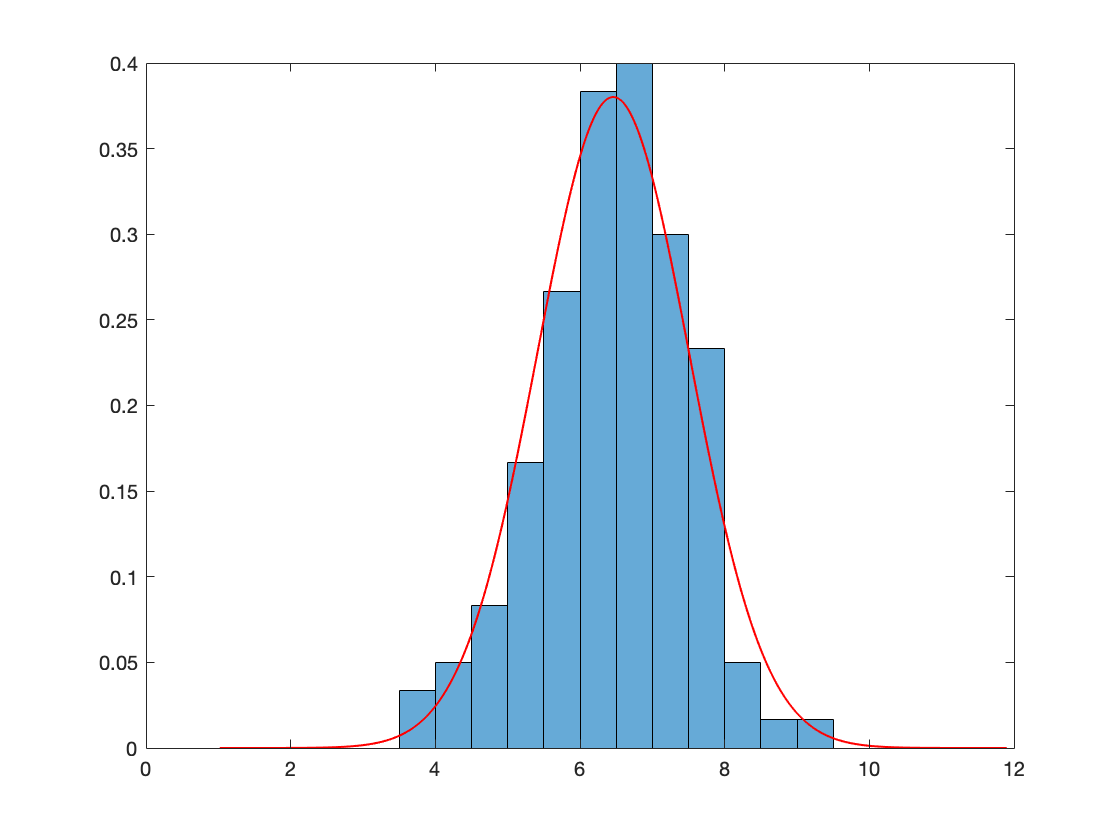
\includegraphics[scale=0.52]{img/Gistogramma.png}
		\caption{Гистограмма}
	\end{figure}

	\newpage
	
	\begin{figure}[H]
		\centering
		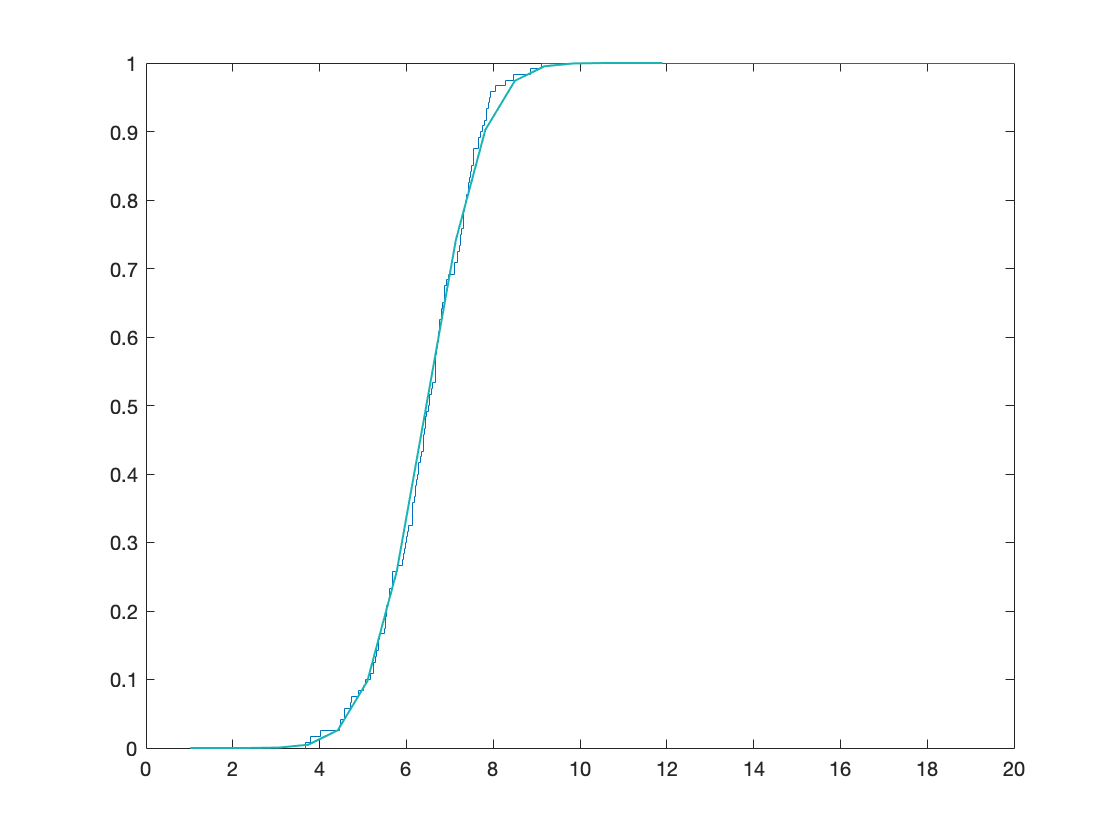
\includegraphics[scale=0.52]{img/EmpericalFunc.png}
		\caption{Эмпирическая функция распределения}
	\end{figure}
	
	
		
	
\end{document}